\documentclass{article}
\usepackage{graphicx} % Required for inserting images

\author{mertyucel}
\date{May 2025}

\usepackage[utf8]{inputenc}
\usepackage{graphicx}
\usepackage{float}
\usepackage{geometry}
\usepackage{hyperref}
\geometry{margin=1in}
\usepackage{enumitem}
\usepackage{amsmath}
\usepackage{graphicx}
\usepackage{titlesec}

\geometry{a4paper, top=1cm, left=2.5cm, right=3cm, bottom=2.0cm}


\begin{document}

\noindent\makebox[\linewidth]{\rule{\paperwidth}{1.5pt}}

\begin{center}
    
\includegraphics[scale=0.0125]{odtu-seeklogo.png} Department of Computer Engineering, METU
\end{center}

\begin{center}
\huge{\textbf{CENG 302}} \\
\Large{Spring 2024-2025} \\
\Large{Homework 3 - SQL} \\
\end{center}


\noindent\makebox[\linewidth]{\rule{\paperwidth}{1.5pt}}

\vspace{0.5mm}

\large{Name, Surname: Mert Yücel}

\large{ID: 2515401}


\section*{Task Solutions}

\begin{text}
    During creating tables and inserting values into the tables, the main problem is that in Character table, there are two guildId values of 0. However, there in no guildId value of 0. Thus, owing to the guildId values in the fourth and fifth rows of Character table, inserting values into tables was not completed, and SQL statements (SELECT FROM's) cannot be run. After adding the fifth question's answer, the problem was solved. The error is below:
\end{text}
\begin{verbatim}
    ERROR:  insert or update on table "character" violates foreign key constraint 
    "character_guildid_fkey"
    Key (guildid)=(0) is not present in table "guild". 

    SQL state: 23503
    Detail: Key (guildid)=(0) is not present in table "guild".
\end{verbatim}


\begin{enumerate}

    \item
    \begin{verbatim}
    SELECT P.playerId
    FROM Player P, Character C, Guild G
    WHERE P.playerId=C.playerId AND C.guildId=G.guildId AND G.guildId=1
    INTERSECT
    SELECT P.playerId
    FROM Player P, Character C, Guild G
    WHERE P.playerId=C.playerId AND C.guildId=G.guildId AND G.guildId=2;
    \end{verbatim}
    \begin{text}
        There is no player that have characters in every guild.
        Cevdet's (11) characters (111 and 116) are in guild 2.
        Seyit's (12) character (112) is in guild 1.
        Arthas' (13) characters (114 and 115) are not in a guild.
        Hekimoğlu's (14) character (113) is in guild 2.
    \end{text}
    \begin{figure}[h]
        \centering
        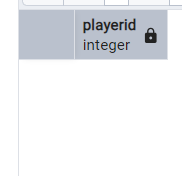
\includegraphics[width=0.25\textwidth]{Ekran Görüntüsü (607).png}
        \caption{Output of the $1^{\text{st}}$ Question}
        \label{fig:ornek}
    \end{figure}
    
\noindent
\vspace{1cm}

    \item
    \begin{verbatim}
    SELECT P3.name
    FROM Player P3
    WHERE P3.playerId IN ((SELECT C.playerId
    FROM Character C
    WHERE C.class='Mage')
    INTERSECT
    (SELECT C2.playerId
    FROM Character C2
    WHERE C2.class='Rogue'));
    \end{verbatim}
    \begin{text}
        There is no player that  have at least one character of class ”Mage” and at least one character of class ”Rogue”. Arthas' (13) character (115) has class ”Mage”. Cevdet's (11) character (111) and Seyit's (12) character (112) have class ”Rogue”. Hence, there is no intersection.
    \end{text}
    \begin{figure}[h]
        \centering
        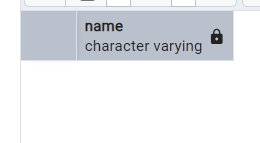
\includegraphics[width=0.25\textwidth]{Ekran Görüntüsü (608).png}
        \caption{Output of the $2^{\text{nd}}$ Question}
        \label{fig:ornek}
    \end{figure}
    
\noindent
\vspace{1cm}

    \item
    \begin{verbatim}
    SELECT C.class, COUNT(QP.status)
    FROM Character C, QuestParticipation QP
    WHERE C.charId=QP.charId AND QP.status='Completed'
    GROUP BY C.class;
    \end{verbatim}

    \begin{figure}[h]
        \centering
        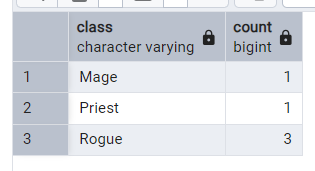
\includegraphics[width=0.25\textwidth]{Ekran Görüntüsü (609).png}
        \caption{Output of the $3^{\text{rd}}$ Question}
        \label{fig:ornek}
    \end{figure}
    
\noindent
\vspace{3cm}

    \item 
    \begin{verbatim}
    SELECT Q.questId, COUNT(DISTINCT C.charId)
    FROM Quest Q, Character C, QuestParticipation QP
    WHERE C.charId=QP.charId AND QP.questId=Q.questId AND Q.questId IN(
    SELECT Q.questId
    FROM Quest Q
    WHERE Q.difficulty='3/5')
    GROUP BY Q.questId
    HAVING COUNT(DISTINCT C.charId) >= 2;
    \end{verbatim}

    \begin{figure}[h]
        \centering
        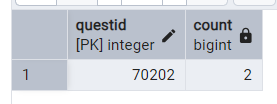
\includegraphics[width=0.25\textwidth]{Ekran Görüntüsü (610).png}
        \caption{Output of the $4^{\text{th}}$ Question}
        \label{fig:ornek}
    \end{figure}
    
\noindent
\vspace{1cm}

    \item
    \begin{verbatim}
    INSERT INTO Guild(guildId, guildName, creationDate) VALUES (0, NULL, NULL);
    \end{verbatim}
    
\vspace{1cm}
\noindent


\end{enumerate}

\begin{center}
    \textit{The entire code block is in the URL of \url{https://github.com/mertyucel02/ceng302_hw3_2515401}}
\end{center}


\end{document}
